\documentclass[11pt]{article}
\usepackage[margin=1in]{geometry}
\usepackage[T1]{fontenc}
\usepackage{lmodern,microtype}
\usepackage{tikz}
\usetikzlibrary{arrows.meta,positioning}
\usepackage[colorlinks=true,urlcolor=blue!45!black,linkcolor=black,citecolor=black]{hyperref}
\hypersetup{pdftitle={Science with Agents},pdfsubject={A lab notebook and scientific ledger for research across AI conversations}}
\usepackage{titlesec}
\titleformat{\section}{\large\bfseries}{\thesection}{.6em}{}
\titleformat{\subsection}{\normalsize\bfseries}{\thesubsection}{.6em}{}
\titlespacing*{\section}{0pt}{1.5ex plus .4ex}{.7ex}
\titlespacing*{\subsection}{0pt}{1.2ex plus .3ex}{.5ex}
\linespread{1.10}
\setlength{\parindent}{1.2em}
\setlength{\parskip}{0pt}
\setlength{\textfloatsep}{10pt plus 2pt minus 2pt}
\begin{document}
\begin{center}
{\LARGE\bfseries Science with Agents}\par\smallskip
{\large A lab notebook for research across AI conversations}
\end{center}
% Abstract written after the body and appendix.
\begin{abstract}
Useful AI conversations often grow into research projects whose assumptions and unfinished work are scattered across interfaces. Science with Agents proposes a small written working agreement around existing tools: give each project a continuing notebook, clear responsibilities, and recoverable saved versions. Its scientific ledger preserves the assumptions, conventions, derivations, inputs, and decisions needed to reconstruct the paper's results. Selected evidence becomes a small companion at submission, with private conversations excluded and checks tied to specific result versions. Researchers choose their own models and execution tools; end-to-end operation remains to be validated.
\end{abstract}

\section{From conversations to a research project}
You ask an AI a question and get a useful answer. You reuse the prompt, follow up on a calculation, and begin to develop a project. Soon one conversation contains a derivation, another a numerical check, and a third the explanation you gave a student. Some work happens in a browser, some through a coding agent, some on a phone. You remember that a sign changed somewhere, but not which convention the latest figure used.

Science with Agents is a proposed working method for this familiar progression. A small set of written rules and ordinary project files gives the work a continuing home. An \emph{agent} is an AI assistant equipped to use tools, such as reading files or running a calculation. The rules tell it how to recover the current question, record a finding, take an assignment, and leave enough evidence for the next conversation. The researcher chooses the model, interface, execution tools, and extent of delegation. The common instructions organize those tools around the project.

The scientific reason for keeping this record extends beyond remembering yesterday's chat. A paper compresses an argument. Its readers must supply background knowledge and often reconstruct intermediate steps. Saving the assumptions and derivations while the research is happening makes that reconstruction easier. The project's notebook connects the day-to-day account to a \emph{scientific ledger}: the dependencies that lead from premises to results. At submission, selected material can accompany the paper, so a colleague can follow a figure back to its calculation without needing the original conversation.

\section{Give the project a continuing home}
\subsection{The project and its notebook}
A project has a folder, a readable front page, and one lab notebook. The notebook states the question, common assumptions and conventions, dated attempts, consequential decisions, and a short account of where work stands. Relevant failures remain in the record. Derivations and outputs have links rather than repeated copies. The scientific ledger lives in these connected records; it needs no separate platform.

Where the interface exposes them, native tool and conversation records are retained privately in a Records folder. The notebook credits people and agents, explains consequential choices, and points to the scientific evidence. An authorized reader can inspect the original exchanges when needed; missing capture remains explicit.

Git keeps recoverable saved versions of files; a \emph{commit} records a meaningful change~\cite{git}. Each project has its own history. GitHub can hold a shared online copy with controlled access. At a milestone, the manager commits the changed files with a scientific task summary, contributors, outcome, and checks. When synchronization is enabled, it also uploads and verifies the checkpoint. The project shows whether work is saved locally or also available online. Personal prompts stay in private conversations, outside this shared account.

\subsection{People, agents, and responsibility}
An agent begins with a recorded identity, project, role, and assignment. \emph{Manager} is a continuing role, held by one conversation at a time. It changes hands only through a recorded handoff, even when several chats read the same instructions.

The record also identifies the models used by the contributing agents. Production and review are credited separately, using model and version information supplied by the application when available. Otherwise the record labels the model unknown or self-reported. This provenance helps a reader decide what needs further checking; a model name cannot certify the science. Reliable identification across interfaces still needs implementation and testing.

The project manager keeps the overall picture, delegates bounded tasks, arranges review, and integrates findings. Several chats can work at once, even on projects with similar names or equations, so each assignment and saved result carries its project identity; overlapping edits still need coordination. Staying inside an assignment is a cooperative rule unless the execution environment enforces it, for example through tool permissions.

With several projects, a central orchestrator relays requests, checks managers, and presents the status and decisions needing the researcher. The managers retain responsibility for execution and review. This division lets the researcher ask for an overview without moving every calculation into one conversation. Colleagues can each use their own agent. Scientific updates and addressed questions in a shared collaboration folder let them work asynchronously; an unanswered question remains visible until its recipient returns.

\subsection{Context and a heartbeat}
A model's \emph{context} is the finite information available for its present work. A long chat may be shortened into a summary, a process called \emph{compaction}, and a fresh chat begins with different context. Continuity therefore depends on reading saved project state. On return or after compaction, the agent recovers its identity and assignment, the current notebook entry, relevant results, and actual outstanding jobs. Checkpoints and checks help detect omissions. Written instructions alone cannot establish that a step was followed.

A \emph{heartbeat} is a periodic check by a lightweight agent. It reads concise manager reports, saved changes, pending reviews, and available usage, then calls the orchestrator when attention is needed. When a check finds no issue, it leaves the orchestrator alone. The heartbeat still costs resources and needs a working scheduler; hard spending limits must come from the execution environment.

\begin{samepage}
An authorized phone interface can read shared records; contacting a running process also requires its host to be available. GitHub holds the uploaded checkpoints. If the usual machine is asleep, another capable environment can continue from the latest verified uploaded checkpoint on a separate branch---a parallel line of saved changes---and reconcile afterward. Changes still confined to the sleeping machine cannot be recovered from GitHub. Setup checks what the chosen browser and other tools can actually read, write, and execute.
\par\end{samepage}

\subsection{Reusable ways of working}
A readable workflow describes a method, its inputs, required checks, and stopping conditions. The researcher can ask to create or adapt one, import a colleague's method, or see which methods are active. One Workflows folder keeps selected methods, skills, and instructions with their origins and versions. Each project selects the methods it needs, including review and cluster procedures. Cross-agent communication instructions are an optional import from the maintained repository. Each Science with Agents invocation checks the relevant instructions for updates and records the version used, preserving active work and local customizations.

Literature searches use the same approach. A researcher can import another group's search workflow and adapt it to a scoped question. By default, the agent suggests running a deep-research task with an available service or equivalent tool. Its output should connect cited findings to source links; key claims are checked against the original papers before entering the notebook and ledger. The saved account distinguishes established results from tentative interpretations and records the search's limits. The provider and workflow can change while these scientific obligations remain.

A group can also reuse a plotting script and style, saving the recipe and input versions beside the figure. SciencePlots supplies an existing collection of plotting styles~\cite{scienceplots}. Reuse preserves presentation choices; correct units, labels, and scientific content still require checking.

\section{The scientific ledger}
\subsection{Unpacking a result}
The scientific ledger is the minimum sufficient record of assumptions, conventions, derivations, inputs, and consequential decisions needed to reconstruct every scientific result in the paper. Common premises are defined once, with explicit exceptions for individual results. What counts as sufficient depends on the stated scientific background and cited sources.

A Fourier-space plot depends on numerical inputs, a calculation, and a derivation with a stated transform convention and boundary assumptions. Figure~\ref{fig:ledger} traces these dependencies; each step carries its version and scientific choices. A discarded normalization that explains an earlier discrepancy also belongs in the record, together with the reason for rejecting it. The consequential decision tree contains this scientific rationale. Private conversation and a model's internal reasoning stay outside it. Shared dependencies can be linked once and used by several results.

\begin{figure}[ht]
\centering
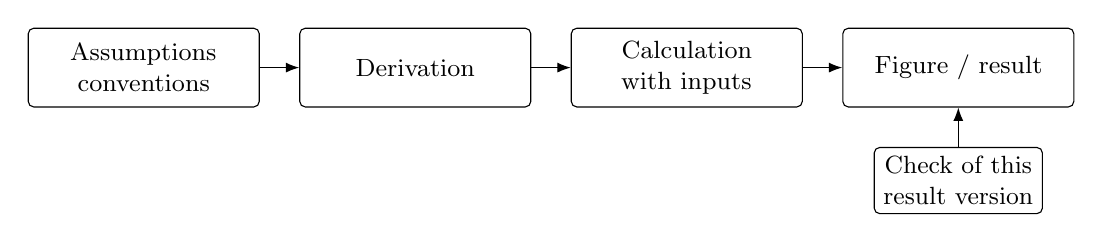
\begin{tikzpicture}[>=Latex,box/.style={draw,rounded corners=2pt,align=center,font=\small,minimum height=10mm,text width=27mm},node distance=5mm]
\node[box] (a) {Assumptions\\conventions};
\node[box,right=of a] (b) {Derivation};
\node[box,right=of b] (c) {Calculation\\with inputs};
\node[box,right=of c] (d) {Figure / result};
\draw[->] (a)--(b);\draw[->] (b)--(c);\draw[->] (c)--(d);
\node[draw,rounded corners=2pt,below=5mm of d,font=\small,align=center] (e) {Check of this\\result version};
\draw[->] (e)--(d);
\end{tikzpicture}
\caption{Follow the arrows backward to unpack a result. Each step carries its scientific choices and exact versions; a check states which result it tests.}
\label{fig:ledger}
\end{figure}

\begin{samepage}
If a boundary assumption changes, these links show which conclusions to revisit. Authorship, cited results, and checks remain distinguishable. A standard theorem can be cited with its conditions; the ledger need not reproduce a textbook.
\par\end{samepage}

\begin{samepage}
Every scientific claim, equation, table, and figure needs a route to stated premises or sources. A missing derivation, unavailable input, or untested step stays an explicit gap. Coverage of the argument, successful reproduction, and correctness are separate questions. A complete record can faithfully preserve an error; a successful rerun can repeat it.
\par\end{samepage}

\subsection{A companion to the paper}
At submission, selected ledger material and evidence form a small folder or ZIP containing derivations, exact inputs and code, outputs, instructions and environment, source attributions, and checks. Ordinary readable files suffice to inspect the scientific account. Standard metadata, such as RO-Crate, can describe the links between these materials~\cite{rocrate}.

Personal prompts and private conversations always stay private; shared notebooks, exported logs, metadata, and commit messages exclude them. The shared material contains scientific premises, methods, and rationale. If an indispensable input cannot be shared, the companion states the resulting reproduction limit. Researchers can publish reusable instruction templates separately.

The baseline is modest: links and files are intact; a recorded check gives its expected and observed outcome; independent reproduction is attempted where feasible. Each check names its scope and exact result version. Failed and contradictory findings remain visible. Numerical checks, human review, and formal proof answer different questions; a proof is conditional on its assumptions. Later tools or verification providers can attach evidence to the same record, preserving the original release and linking additions to the versions they assess. Clear local definitions could later connect to a proposed broader physics graph, with results as nodes and mathematical operations as edges; that integration remains unimplemented.

\section{Beginning with an existing project}
Begin with ``Use Science with Agents'' in your preferred agent, using \href{https://sciencewithagents.com}{\mbox{sciencewithagents.com}} as the entry point. Setup first finds any existing workspace and manager, then recovers the assignment or arranges an explicit handoff. A fresh setup copies the shared instruction repository, connects the user's GitHub account, and establishes project storage and execution tools. The agent guides the process through conversation, screenshots, or supported browser access; maintained documentation gives the current routes.

One \emph{My Projects} home lists new projects and links existing projects in place. New projects receive their own history; adopted projects keep their existing work. Ask for help or a list of active methods.

Companion packaging has been tested on synthetic examples. End-to-end capture, cross-interface participation, and provider integrations remain to be validated. A researcher can begin with one question and its current assumptions, ask the agent to keep the notebook, and review the first saved finding. That entry gives a returning colleague or student a place to learn how the result was obtained.

\clearpage
\appendix
\section{A derivation, a cluster run, and a colleague's return}
Consider an illustrative collaboration. A develops the theory; B has already configured successful cluster runs. While B is away, A changes a normalization. The notebook identifies the adopted convention, affected results, B's saved method, and jobs already running.

A's own identified agent follows the imported cluster workflow. It compares the proposed run with the established partition, requested resources, environment, permitted scope, and existing jobs. Within those bounds, it can submit using A's authorized access. The job receipt records submission; any required scientific review remains pending. An action requiring B's answer waits while independent work continues.

The record connects the changed convention and derivation to the job receipt, observed result, and a numerical check with stated tolerance. The check specifies which quantities should change and which should remain invariant under the revised convention. The figure uses an imported plotting recipe, saved with its inputs. A milestone commit links the scientific task summary and contributors to these changes and their evidence. If an output expected to change retains its old value, the discrepancy is recorded and investigated before the new figure is accepted.

A leaves an addressed, nonurgent question in the shared collaboration folder: does the revised normalization require changing the comparison observable too? Later B opens an authorized chat, recovers the project record, sees the changed derivation and pending question, and replies. Existing jobs are inspected before any repeat submission. B's answer and resulting correction receive their own saved record, so the reason for the final convention remains recoverable.

At submission, this same derivation, run, and figure enter the scientific companion. Unperformed checks and unanswered questions remain visible. A reader can follow the published curve to the inputs, the calculation, and the normalization decision, then contribute another check tied to the released result.

\begin{thebibliography}{9}
\small
\bibitem{git} S. Chacon and B. Straub, \emph{Pro Git}, ``Getting Started: What is Git?'' \href{https://git-scm.com/book/en/v2/Getting-Started-What-is-Git\%3F}{git-scm.com/book}.
\bibitem{scienceplots} SciencePlots contributors, \href{https://scienceplots.readthedocs.io/en/sphinx-documentation/guides/getting_started.html}{\emph{SciencePlots: Getting started}}.
\bibitem{rocrate} RO-Crate community, \href{https://www.researchobject.org/ro-crate/specification/1.3/index.html}{\emph{RO-Crate specification 1.3}}.
\end{thebibliography}
\end{document}
